%\hypertarget{___gatsby}{}
%\hypertarget{gatsby-focus-wrapper}{}
%\href{https://mukulrathi.com/}{}
%
%MUKUL RATHI
%
%\href{https://mukulrathi.com/about-me}{}
%
%About Me
%
%\href{https://mukulrathi.com/blog}{}
%
%Blog
%
%\hypertarget{creating-the-bolt-compiler-part-4}{%
%\subsection{Creating the Bolt Compiler: Part
%4}\label{creating-the-bolt-compiler-part-4}}

\hypertarget{top-of-page}{%
\chapter{An accessible introduction to type theory and implementing a
type-checker}\label{top-of-page}}

June 15, 2020

%\hypertarget{june-15-2020}{%
%\subsection{June 15, 2020}\label{june-15-2020}}
%
%\hypertarget{min-read}{%
%\subsection{11 min read}\label{min-read}}
%
%\hypertarget{last-updated-january-13-2021}{%
%\subsection{Last updated: January 13,
%2021}\label{last-updated-january-13-2021}}
%
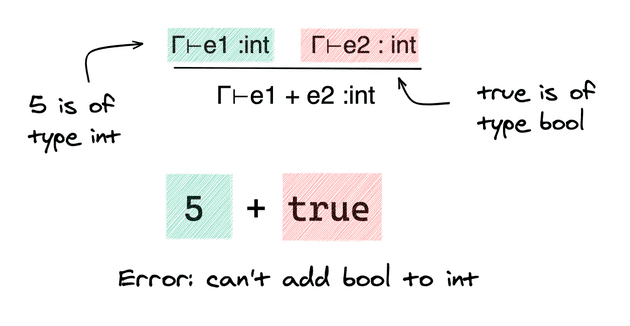
\includegraphics[width=\linewidth]{04_files/type-check.png}
%
%\hypertarget{series-creating-the-bolt-compiler}{%
%\section{Series: Creating the Bolt
%Compiler}\label{series-creating-the-bolt-compiler}}
%
%\begin{itemize}
%\item
%  { Part 1:
%  }\href{https://mukulrathi.com/create-your-own-programming-language/intro-to-compiler/}{How
%  I wrote my own "proper" programming language}
%\item
%  { Part 2:
%  }\href{https://mukulrathi.com/create-your-own-programming-language/compiler-engineering-structure/}{So
%  how do you structure a compiler project?}
%\item
%  { Part 3:
%  }\href{https://mukulrathi.com/create-your-own-programming-language/parsing-ocamllex-menhir/}{Writing
%  a Lexer and Parser using OCamllex and Menhir}
%\item
%  \textbf{Part 4: An accessible introduction to type theory and
%  implementing a type-checker}
%\item
%  { Part 5:
%  }\href{https://mukulrathi.com/create-your-own-programming-language/data-race-dataflow-analysis/}{A
%  tutorial on liveness and alias dataflow analysis}
%\item
%  { Part 6:
%  }\href{https://mukulrathi.com/create-your-own-programming-language/lower-language-constructs-to-llvm/}{Desugaring
%  - taking our high-level language and simplifying it!}
%\item
%  { Part 7:
%  }\href{https://mukulrathi.com/create-your-own-programming-language/protobuf-ocaml-cpp-tutorial/}{A
%  Protobuf tutorial for OCaml and C++}
%\item
%  { Part 8:
%  }\href{https://mukulrathi.com/create-your-own-programming-language/llvm-ir-cpp-api-tutorial/}{A
%  Complete Guide to LLVM for Programming Language Creators}
%\item
%  { Part 9:
%  }\href{https://mukulrathi.com/create-your-own-programming-language/concurrency-runtime-language-tutorial/}{Implementing
%  Concurrency and our Runtime Library}
%\item
%  { Part 10:
%  }\href{https://mukulrathi.com/create-your-own-programming-language/generics-parametric-polymorphism/}{Generics
%  - adding polymorphism to Bolt}
%\item
%  { Part 11:
%  }\href{https://mukulrathi.com/create-your-own-programming-language/inheritance-method-overriding-vtable/}{Adding
%  Inheritance and Method Overriding to Our Language}
%\end{itemize}
%
%\begin{center}\rule{0.5\linewidth}{0.5pt}\end{center}

This post is split into 2 halves: the first half explains the theory
behind type-checkers, and the second half gives you a detailed deep-dive
into how it's implemented in our compiler for our language Bolt. Even if
you aren't interested in writing your own language, the first half is
useful if you've ever heard about \emph{type systems} and want to know
how they even work!

%\hypertarget{share-this-on-twitter}{%
%\subsection{Share This On Twitter}\label{share-this-on-twitter}}
%
%If you find this useful, please share this on Twitter. I'm writing up
%posts on implementing generics and inheritance in this language too!
%
%\includegraphics[width=1.04167in,height=1.11458in]{04_files/profile-pic_004.png}

\hypertarget{what-are-types}{%
\section{\texorpdfstring{\protect\hyperlink{what-are-types}{}What are
types?}{What are types?}}\label{what-are-types}}

We'd discussed this briefly in the first part of the compiler series,
however let's revisit this:

Types are a way of \emph{grouping} program values based on the
\emph{behaviour} we'd like them to have. We have our own ``types'' in
our day-to-day lives. E.g. grouping people as \emph{adults} and
\emph{children}.

Grouping values together means the compiler doesn't have as many cases
to handle. It means we don't need to look at the \emph{actual value}, we
just reason about it based on the \emph{group} it's in (its type).

E.g. the values \texttt{0}, \texttt{1}, \texttt{2}, \texttt{3}\ldots{}
and all other integers are all given the type \texttt{int}. Values of
type \texttt{int} can take part in arithmetic operations like
multiplication on them but we can't concatenate them (like
\texttt{string}s). See how the type (\texttt{int} vs \texttt{string})
defines the \emph{behaviour} of the value (what we can do with them)?

It's even clearer in our custom types. E.g when you define a custom
\texttt{Animal} class with \texttt{eat()} and \texttt{sleep()} methods,
you're saying that objects of type \texttt{Animal} have \texttt{eat} and
\texttt{sleep} behaviour. But we can't divide two \texttt{Animal}
objects by each other - that's not the behaviour we'd allow. What would
\texttt{dog\ /\ cat} even mean?

The role of the \textbf{type-checker} is to prevent this kind of
nonsensical behaviour from happening. That's what we're building today.

All practical languages have type-checking in some form.
\textbf{Statically} typed languages like Rust, Java or Haskell check the
types at \emph{compile-time}. Dynamically-typed languages like JS and
Python \textbf{do} still have types - values are tagged with types at
runtime, and they check types when executing. If you try to run
\texttt{5\ /\ "Hello"}, it won't actually run the code, JS/Python will
see \texttt{"Hello} has type \texttt{string} and will throw a runtime
error instead of executing it.

Right now, this all feels a little hand-wavey. Let's formalise
``preventing nonsensical behaviour''. We want a list of rules to check a
program against, and then if it passes those, we know our program is
safe.

This collection of rules is called a \emph{type system}.

\hypertarget{type-systems}{%
\section{\texorpdfstring{\protect\hyperlink{type-systems}{}Type
Systems}{Type Systems}}\label{type-systems}}

Here's the deal: types define \emph{safe behaviour}. So if we can give
an expression a type, we can use its type to make sure it's being used
in the correct way. The type system's rules (called \emph{typing
judgements}) therefore try to assign a type {{{\(t\)}{{{}{t}}}}} to an
expression {{{\(e\)}{{{}{e}}}}}.

We start by defining seemingly obvious facts, like \texttt{true} is of
type bool. In our type system, the rule is written as follows:

{{\ignoresecond{\(\vdash {\mathbf{t}\mathbf{r}\mathbf{u}\mathbf{e}}:bool\)}{{{}{⊢}{}}{{}{{true}}{}{:}{}}{{}{b}{oo}{l}}}}}

Don't be scared by the maths notation: {{\ignoresecond{\(\vdash\)}{{{}{⊢}}}}} means
``it follows that''. You can read this as ``it follows that the
expression \texttt{true} has type \texttt{bool}. In general,
{{\ignoresecond{\(\vdash \mathbf{e}:t\)}{{{}{⊢}{}}{{}{e}{}{:}{}}{{}{t}}}}} can be
read as ``it follows that expression e has type t''.

Here's a couple more obvious facts.

{{\ignoresecond{\(\vdash {\mathbf{f}\mathbf{a}\mathbf{l}\mathbf{s}\mathbf{e}}:bool\)}{{{}{⊢}{}}{{}{{false}}{}{:}{}}{{}{b}{oo}{l}}}}}

{{\ignoresecond{\(\vdash n:int\)}{{{}{⊢}{}}{{}{n}{}{:}{}}{{}{in}{t}}}}} for any
integer {{{\(n\)}{{{}{n}}}}}.

\hypertarget{typing-environments}{%
\subsection{\texorpdfstring{\protect\hyperlink{typing-environments}{}Typing
environments}{Typing environments}}\label{typing-environments}}

Thing is, looking at an expression on its own isn't always enough for us
to type-check it. What's the type of a variable \texttt{x}? What should
we put in place of the \texttt{?} below?

{{\ignoresecond{\(\vdash x:\ ?\)}{{{}{⊢}{}}{{}{x}{}{:}{~}}{{}{?}}}}}

Well it depends on what type it was given when it was defined. So when
type-checking, we'll need to keep track of the variables' types as they
are defined. We call this the \emph{typing environment}, represented in
our rules as {{\ignoresecond{\(\Gamma\)}{{{}{Γ}}}}} . Think of
{{\ignoresecond{\(\Gamma\)}{{{}{Γ}}}}} as a look-up function that maps variables to
their types.

We update our typing rules to include {{{\(\Gamma\)}}}:

{{{\(\Gamma \vdash \mathbf{x}:t\)}}}.

Back to our typing rule here:

{{{\(\Gamma \vdash x:\ ?\)}}}

\emph{If} {{{\(\Gamma(x) = t\)}},
\emph{then} we can say that:

{{{\(\Gamma \vdash \mathbf{x}:t\)}}}.

In our typing rules we stack these two statements to give one compound
typing rule for variables. This is an example of an \emph{inference}
rule.

{{{\(\frac{\Gamma(x) = t}{\Gamma \vdash x:\ t}\)}}}

\hypertarget{inference-rules}{%
\subsection{\texorpdfstring{\protect\hyperlink{inference-rules}{}Inference
rules}{Inference rules}}\label{inference-rules}}

This odd stacked ``fraction'' is a way of representing deductive
reasoning (like Sherlock Holmes!). If everything on the top holds, then
we \emph{infer} the bottom also holds.

Here's another rule. This says that if we know
{{{\(e_{1}\)}}} and
{{{\(e_{2}\)}}} are
\texttt{int}s, then if we add them together the result is also an
\texttt{int}.

{{\(\frac{\Gamma \vdash e_{1}:int\text{~~~~~~}\Gamma \vdash e_{2}:int}{\Gamma \vdash e_{1} + e_{2}:\ int}\)}}

Using these \emph{inference} rules, we can stack together our pieces of
evidence about different parts of the program to reason about the whole
program. This is how we build up our type system - we \emph{stack} our
rules.

Let's combine what we've learnt so far to type-check a little
expression: \texttt{x\ +\ 1} where our environment
{{{\(\Gamma\)}}} tells us \texttt{x} is an \texttt{int}.

{{{\(\frac{\frac{\frac{}{\Gamma(x) = int}}{\Gamma \vdash x:\ int}\text{~~~~~~}\frac{}{\Gamma \vdash 1:\ int}}{\Gamma \vdash x + 1:\ int}\)}}

Now if it turns out \texttt{x} is an \texttt{string}, then
{{{\(\Gamma(x) = int\)}}} doesn't
hold, so all the rules stacked below it don't hold. Our type-checker
would raise an \emph{error}, as the types don't match up!

\hypertarget{axioms}{%
\subsection{\texorpdfstring{\protect\hyperlink{axioms}{}Axioms}{Axioms}}\label{axioms}}

It's convention here to represent the facts (\emph{axioms}) with a line
above them. You can think them as the ``base case'':

{{{\(\frac{}{\Gamma \vdash 1:\ int}\)}}}

Since they have nothing on the top, technically everything on the top is
true. So the bottom \textbf{always} holds.

If you look back to our example and flip it upside down, it kind of
looks like a tree. It also lays out our reasoning, so acts as a
\emph{proof} - you can just follow the steps. Why is \texttt{x+1} an
int? Well \texttt{x} and \texttt{1} are \texttt{int}s? Why is \texttt{x}
an int? Because\ldots{} You get the idea. So what we've constructed here
is called a \emph{proof tree}.

Okay, let's look at another rule. What about an \texttt{if-else} block?

%Copy

\begin{verbatim}
if (something) {  do_one_thing} else {  do_something_else}
\end{verbatim}

Well, the \texttt{something} has to have type \texttt{bool} as it's a
condition. What about the branches? We need to give this expression an
overall type, but because we're \emph{statically} type-checking, we
don't know which branch will be executed at runtime. Therefore we need
both branches to return the \textbf{same type} (call it
{{{\(t\)}{{{}{t}}}}}), so the expression has the same type
\emph{regardless} of which branch we execute.

{{{\(\frac{\Gamma \vdash e_{1}:bool\text{~~~~~~}\Gamma \vdash e_{2}:t\text{~~~~~~}\Gamma \vdash e_{3}:t}{\Gamma \vdash {\mathbf{i}\mathbf{f}}\ e_{1}\ \{ e_{2}\}\ {\mathbf{e}\mathbf{l}\mathbf{s}\mathbf{e}}\ \{ e_{3}\}:\ t}\)}}}

JavaScript and Python \textbf{would} allow different types for each
branch, since they're doing their type-checking at runtime
(\emph{dynamically} typed), so they know which branch was chosen.

\hypertarget{typing-the-overall-program}{%
\subsection{\texorpdfstring{\protect\hyperlink{typing-the-overall-program}{}Typing
the Overall
Program}{Typing the Overall Program}}\label{typing-the-overall-program}}

This post would end up being too long if I were to list all the rules,
but you can work through each of the cases. We look at the
\emph{grammar} we defined in the previous post and write the
corresponding rules.

We want to show the program is \emph{well-typed} (you can assign it a
type) to show it is safe. So we essentially want a proof tree that shows
it has some type {{{\(t\)}{{{}{t}}}}} (we don't care which):

{{\(\{\}\  \vdash program:\ t\)}}

There's just one thing missing here. Initially
{{{\(\Gamma = \{\}\)}}} - it's empty as we
haven't defined any variables. How do we \textbf{add variables} to
{{\(\Gamma\)}}?

Remember, we add variables to {{{\(\Gamma\)}}} as we declare
them in our program. The syntax for this is a \texttt{let} declaration.
So say we have the following program:

%Copy

\begin{verbatim}
// we have some gamma
let x = e1
// update gamma with x's type
// continue type-checking
e2
\end{verbatim}

We type-check this in the order the program executes:

\begin{itemize}
\tightlist
\item
  We get the type of the expression
  {{\ignoresecond{\(e_{1}\)}{{{}{{e}{{{{{{}{{1}}}}{\hspace{0pt}}}{{{}}}}}}}}}} , call
  it {{{\(t1\)}{{{}{t}{1}}}}}
\item
  We then \emph{extend} the environment {{\ignoresecond{\(\Gamma\)}{{{}{Γ}}}}} with
  the new mapping
  {{\ignoresecond{\(x:t_{1}\)}{{{}{x}{}{:}{}}{{}{{t}{{{{{{}{{1}}}}{\hspace{0pt}}}{{{}}}}}}}}}}.
\item
  We use this extended environment (which we write as
  {{\ignoresecond{\(\Gamma,x:t_{1}\)}{{{}{Γ}{,}{}{x}{}{:}{}}{{}{{t}{{{{{{}{{1}}}}{\hspace{0pt}}}{{{}}}}}}}}}}
  ) to type-check
  {{\ignoresecond{\(e_{2}\)}{{{}{{e}{{{{{{}{{2}}}}{\hspace{0pt}}}{{{}}}}}}}}}} and
  give it type
  {{\ignoresecond{\(t_{2}\)}{{{}{{t}{{{{{{}{{2}}}}{\hspace{0pt}}}{{{}}}}}}}}}}.
\end{itemize}

The whole typing rule thus looks like:

{{\ignoresecond{\(\frac{\Gamma \vdash e_{1}:t_{1}\text{~~~~~}\Gamma,x:t_{1} \vdash e_{2}:t_{2}}{\Gamma \vdash {\mathbf{l}\mathbf{e}\mathbf{t}}\ x = e_{1};\ e_{2}:t_{2}}\)}{{{}{{}{{{{{{}{{Γ}{}{⊢}{}{{let}}{~}{x}{}{=}{}{{e}{{{{{{}{{1}}}}{\hspace{0pt}}}{{{}}}}}}{;}{~}{}{{e}{{{{{{}{{2}}}}{\hspace{0pt}}}{{{}}}}}}{}{:}{}{{t}{{{{{{}{{2}}}}{\hspace{0pt}}}{{{}}}}}}}}{{}{}}{{}{{Γ}{}{⊢}{}{{e}{{{{{{}{{1}}}}{\hspace{0pt}}}{{{}}}}}}{}{:}{}{{t}{{{{{{}{{1}}}}{\hspace{0pt}}}{{{}}}}}}{~}{~}{~}{~}{~}{Γ}{,}{}{x}{}{:}{}{{t}{{{{{{}{{1}}}}{\hspace{0pt}}}{{{}}}}}}{}{⊢}{}{{e}{{{{{{}{{2}}}}{\hspace{0pt}}}{{{}}}}}}{}{:}{}{{t}{{{{{{}{{2}}}}{\hspace{0pt}}}{{{}}}}}}}}}{\hspace{0pt}}}{{{}}}}}{}}}}}}

\hypertarget{type-checking-vs-type-inference}{%
\subsection{\texorpdfstring{\protect\hyperlink{type-checking-vs-type-inference}{}Type
Checking vs Type
Inference}{Type Checking vs Type Inference}}\label{type-checking-vs-type-inference}}

One finer point: here we wrote \texttt{let\ x\ =\ e}. We could have
equally written this as \texttt{let\ x\ :\ t\ =\ e} - where the
programmer \emph{annotates} \texttt{x} with type \texttt{t}. e.g.
\texttt{let\ x\ :\ int\ =\ 1\ +\ 2}.

These lead to different typing algorithms - in the first case the
compiler \emph{infers} that \texttt{1+2} has type \texttt{int}, and in
the second case, the compiler has to \emph{check} that \texttt{1+2} has
type \texttt{int} (since we specified the type \texttt{int} of
\texttt{x}).

As you might imagine, type inference means that the programmer has to
write fewer type annotations, but it is much more complex for the
compiler - it's like filling a Sudoku from scratch versus checking a
Sudoku solution is valid. OCaml and Haskell are examples of languages
with type inference baked in.

In practice, most statically-typed languages do require some type
annotations, but can infer some types (e.g. the \texttt{auto} keyword in
C++). This is like completing a partially solved Sudoku puzzle and is
much easier.

For Bolt, we're going to infer types \emph{within} a function or method
definition, but require programmers to annotate the parameter and return
types. This is a nice middle ground.

%{example\_function.bolt}

%Copy

\begin{verbatim}
function int something(int x, bool y){
  let z = ...
 // z's type is inferred
  ...
}
\end{verbatim}

Okay, enough theory, let's get to implementing this type-checker!

%\hypertarget{i-make-content-about-my-software-engineering-journey-curated-in-my-newsletter}{%
%\subsection{I make content about my software engineering journey,
%curated in my
%newsletter!}\label{i-make-content-about-my-software-engineering-journey-curated-in-my-newsletter}}
%
%Want to learn about how more advanced language features like generics
%and inheritance are typed? Subscribe to receive *exclusive* access to
%future posts before they're released to the general internet.
%
%\href{https://newsletter.mukulrathi.com/}{Check out previous issues!}
%
%Email Address
%
%By subscribing, you agree with Revue's
%\href{https://www.getrevue.co/terms}{Terms of Service} and
%\href{https://www.getrevue.co/privacy}{Privacy Policy}.

\hypertarget{implementing-a-type-checker}{%
\section{\texorpdfstring{\protect\hyperlink{implementing-a-type-checker}{}Implementing
a
Type-checker}{Implementing a Type-checker}}\label{implementing-a-type-checker}}

\hypertarget{just-give-me-the-code}{%
\subsection{\texorpdfstring{\protect\hyperlink{just-give-me-the-code}{}Just
give me the
code!}{Just give me the code!}}\label{just-give-me-the-code}}

You'll need to clone the Bolt repository:

%Copy

\begin{verbatim}
git clone https://github.com/mukul-rathi/bolt
\end{verbatim}

The \href{https://github.com/mukul-rathi/bolt}{Bolt repository}
\texttt{master} branch contains a more complex type-checker, with
support for inheritance, function/method overloading and generics. Each
of these topics will get its own special post later in the series.

So instead, you'll want to look at the \texttt{simple-compiler-tutorial}
release. You can do this as follows:

%Copy

\begin{verbatim}
git checkout simple-compiler-tutorial
\end{verbatim}

This contains a stripped-back version of Bolt from earlier in the
development processs.
\href{https://github.com/mukul-rathi/bolt/tree/simple-compiler-tutorial}{(View
this online)}

The folder we care about is \texttt{src/frontend/typing}.

\hypertarget{a-note-on-ocaml-syntax}{%
\subsection{\texorpdfstring{\protect\hyperlink{a-note-on-ocaml-syntax}{}A
note on OCaml
syntax}{A note on OCaml syntax}}\label{a-note-on-ocaml-syntax}}

In this tutorial we'll be using OCaml syntax. If you're unfamiliar with
this, the main gist is that we'll:

\textbf{a)} Pattern match each of the cases (like \texttt{switch}
statements in other languages). Here we have a variable \texttt{x} and
we do different things based on each of its cases \texttt{A}, \texttt{B}

%Copy

\begin{lstlisting}[language=caml]
match x with  | A -> something  | B -> something_else
\end{lstlisting}

\textbf{b)} Use a Result monad: in essence, this has two values:
\texttt{Ok\ something} and \texttt{Error}. We sequence each of the
operations using the \texttt{\textgreater{}\textgreater{}=} operator -
you don't need to know anything about monads for this tutorial, just
think of this as the same as normal expression sequencing with
\texttt{;}s, just that we're using another operator to represent that
earlier expressions might raise an error.

\hypertarget{types-in-bolt}{%
\subsection{\texorpdfstring{\protect\hyperlink{types-in-bolt}{}Types
in Bolt}{Types in Bolt}}\label{types-in-bolt}}

Bolt has four main types: \texttt{int}, \texttt{bool}, \texttt{void} and
user-defined classes. We represent these four options using a variant
type \texttt{type\_expr} in OCaml:

%{
%\href{https://github.com/mukul-rathi/bolt/blob/simple-compiler-tutorial/src/frontend/ast/ast_types.mli}{ast\_types.mli}}
%
%Copy

\begin{lstlisting}[language=caml,caption={ast\_types.mli}]
type type_expr = TEInt | TEClass of Class_name.t | TEVoid | TEBool
\end{lstlisting}

\hypertarget{annotating-our-ast-with-types}{%
\subsection{\texorpdfstring{\protect\hyperlink{annotating-our-ast-with-types}{}Annotating
our AST with
types}{Annotating our AST with types}}\label{annotating-our-ast-with-types}}

Let's recap our Abstract Syntax Tree from the last part of the series:

%{
%\href{https://github.com/mukul-rathi/bolt/blob/simple-compiler-tutorial/src/frontend/parsing/parsed_ast.mli}{parsed\_ast.mli}}
%
%Copy

\begin{lstlisting}[caption={parsed\_ast.mli},language=caml]
type identifier =
  | Variable of Var_name.t (* x *)
  | ObjField of Var_name.t * Field_name.t (* x.f *)

type expr =
  | Integer     of loc * int (* 1, 2 *)
  | Boolean     of loc * bool (* true*)
  | Identifier  of loc * identifier
  | Constructor of loc * Class_name.t * constructor_arg list (* new Class(args)*)
  | Let         of loc * type_expr option * Var_name.t * expr
    (** let x = e (optional type annotation) *)
  | Assign      of loc * identifier * expr
  | If          of loc * expr * block_expr * block_expr
    (** If ___ then ___ else ___ *)
  ...

and block_expr = Block of loc * expr list
\end{lstlisting}

This AST annotates each expression with \texttt{loc} - the line and
position of the expression. In our type-checking phase, we'll be
checking the types of each of the possible expressions. We'll want to
store our results by \emph{directly annotating} the AST, so the next
compiler stage can view the types just by looking at the AST.

This AST gets the imaginative name \texttt{typed\_ast}:

%{
%\href{https://github.com/mukul-rathi/bolt/blob/simple-compiler-tutorial/src/frontend/typing/typed_ast.mli}{typed\_ast.mli}}
%
%Copy

\begin{lstlisting}[caption={typed\_ast.mli},language=caml]
type identifier =
  | Variable of type_expr * Var_name.t
  | ObjField of Class_name.t * Var_name.t * type_expr * Field_name.t
      (** class of the object, type of field *)

type expr =
  | Integer     of loc * int  (** no need to annotate as obviously TEInt *)
  | Boolean     of loc * bool  (** no need to annotate as obviously TEBool *)
  | Identifier  of loc * identifier  (** Type info associated with identifier *)
  | Constructor of loc * type_expr * Class_name.t * constructor_arg list
  | Let         of loc * type_expr * Var_name.t * expr
  | Assign      of loc * type_expr * identifier * expr
  | If          of loc * type_expr * expr * block_expr * block_expr
      (** the If-else type is that of the branch exprs *)
  ...

and block_expr =
  | Block of loc * type_expr * expr list  (** type is of the final expr in block *)
\end{lstlisting}

We don't annotate obvious types, like for \texttt{Integer} and
\texttt{Boolean}, but we annotate the type of the overall expression for
other expressions e.g. the type returned by an \texttt{if-else}
statement.

A good rule of thumb when annotating the AST is, what would the next
stage need to be told about the program that it can't guess from it
being well-typed? For an \texttt{if-else} statement, if it is well-typed
then the if-condition expression is clearly of type \texttt{bool}, but
we'd need to be told the type of the branches.

\hypertarget{the-type-environment}{%
\subsection{\texorpdfstring{\protect\hyperlink{the-type-environment}{}The
Type Environment}{The Type Environment}}\label{the-type-environment}}

Recall that we used our type environment {{\ignoresecond{\(\Gamma\)}{{{}{Γ}}}}} to
look up the types of variables. We can store this as a list of
\emph{bindings} (variable, type) pairs.

\texttt{type\_env.ml} also contains a ``environment'' of helper
functions that we'll use in this type-checking phase. These are mostly
uninteresting getter methods that you can look at in the repo.

%{
%\href{https://github.com/mukul-rathi/bolt/blob/simple-compiler-tutorial/src/frontend/typing/type_env.mli}{type\_env.mli}}
%
%Copy
\begin{lstlisting}[language=caml,caption={type\_env.mli}]
type type_binding = Var_name.t * type_expr
type type_env = type_binding list

(** A bunch of getter methods used in type-checking the core language *)
val get_var_type : Var_name.t -> type_env -> loc -> type_expr Or_error.t
\end{lstlisting}

It also includes a couple of functions that check we can assign to an
identifier (it's not \texttt{const} or the special identifier
\texttt{this}) and that check we don't have duplicate variable
declarations (shadowing) in the same scope. These again are conceptually
straightforward but are necessary just to cover edge cases.

For example:

\begin{lstlisting}[language=caml,caption={type\_env.ml}]
let check_identifier_assignable class_defns id env loc =
  let open Result in
  match id with
  | Parsed_ast.Variable x ->
      if x = Var_name.of_string "this" then
        Error
          (Error.of_string
             (Fmt.str "%s Type error - Assigning expr to 'this'.@." (string_of_loc loc)))
      else Ok ()
  | Parsed_ast.ObjField (obj_name, field_name) ->
      get_obj_class_defn obj_name env class_defns loc
      >>= fun class_defn ->
      get_class_field field_name class_defn loc
      >>= fun (TField (modifier, _, _, _)) ->
      if modifier = MConst then
        Error
          (Error.of_string
             (Fmt.str "%s Type error - Assigning expr to a const field.@."
                (string_of_loc loc)))
      else Ok ()


\end{lstlisting}

\hypertarget{typing-expressions}{%
\subsection{\texorpdfstring{\protect\hyperlink{typing-expressions}{}Typing
Expressions}{Typing Expressions}}\label{typing-expressions}}

This. This is the \emph{crux} of the implementation. So if you've been
skimming the post, here's where you should pay attention.

What do we need to type-check an expression?

We need the class definitions and function definitions, in case we need
to query the types of fields and function/method type signatures. We
also need the expression itself, and the typing environment we're using
to type-check it.

What do we return? The typed expression, along with its type (we return
type separately to make recursive calls more straightforward). Or we
return an error, if the expression is not well-typed.

Our function type signature captures this exactly:

%{
%\href{https://github.com/mukul-rathi/bolt/blob/simple-compiler-tutorial/src/frontend/typing/type_expr.mli}{type\_expr.mli}}
%
%Copy

\begin{lstlisting}[language=caml,caption={type\_expr.mli}]
val type_expr :
     Parsed_ast.class_defn list
  -> Parsed_ast.function_defn list
  -> Parsed_ast.expr
  -> type_env
  -> (Typed_ast.expr * type_expr) Or_error.t
\end{lstlisting}

In the
\href{https://mukulrathi.com/create-your-own-programming-language/compiler-engineering-structure/}{second
post} in this series, I discussed why we're using OCaml. This stage of
the compiler is one where it really pays off.

For example to type an identifier, we pattern match based on whether it
is a variable \texttt{x} or an object field \texttt{x.f}. If it is a
variable then we get its type from the environment (we pass in
\texttt{loc} as line+position info for error messages). If it returns a
\texttt{var\_type} without an error, then we return the type-annotated
variable.

If it is an object field \texttt{x.f}, then we need to look up the type
of object \texttt{x} in the \texttt{env} and get its corresponding class
definition. We can then look up the type of field \texttt{f} in the
class definition. Then we annotate the identifier with the two bits of
type information we've just learnt: the class of the object, and the
field type.

Our code does exactly that, with no boilerplate:

%{
%\href{https://github.com/mukul-rathi/bolt/blob/simple-compiler-tutorial/src/frontend/typing/type_expr.ml}{type\_expr.ml}}
%
%Copy
\begin{lstlisting}[language=caml,caption={{type\_expr.ml}}]
let type_identifier class_defns identifier env loc =
  let open Result in
  match identifier with
    | Parsed_ast.Variable var_name ->
      get_var_type var_name env loc
      >>| fun var_type -> (Typed_ast.Variable (var_type, var_name), var_type)
  | Parsed_ast.ObjField (var_name, field_name) ->
      get_obj_class_defn var_name env class_defns loc
      >>= fun (Parsed_ast.TClass (class_name, _, _, _) as class_defn) ->
      get_class_field field_name class_defn loc
      >>| fun (TField (_, field_type, _, _)) ->
      (Typed_ast.ObjField (class_name, var_name, field_type, field_name), field_type)
\end{lstlisting}
%\begin{verbatim}
%let type_identifier class_defns identifier env loc =  let open Result in  match identifier with    | Parsed_ast.Variable var_name ->      get_var_type var_name env loc      >>| fun var_type -> (Typed_ast.Variable (var_type, var_name), var_type)  | Parsed_ast.ObjField (var_name, field_name) ->      get_obj_class_defn var_name env class_defns loc      >>= fun (Parsed_ast.TClass (class_name, _, _, _) as class_defn) ->      get_class_field field_name class_defn loc      >>| fun (TField (_, field_type, _, _)) ->      (Typed_ast.ObjField (class_name, var_name, field_type, field_name), field_type)
%\end{verbatim}

Right, so let's look at expressions. This again is clean code that just
reads like our typing judgements. We have \texttt{expr1\ binop\ expr2}
where \texttt{expr1} and \texttt{expr2} are being combined using some
binary operator e.g. \texttt{+}.

Let's remind ourselves of the rule:

{{\ignoresecond{\(\frac{\Gamma \vdash e_{1}:int\text{~~~~~~}\Gamma \vdash e_{2}:int}{\Gamma \vdash e_{1} + e_{2}:\ int}\)}{{{}{{}{{{{{{}{{Γ}{}{⊢}{}{{e}{{{{{{}{{1}}}}{\hspace{0pt}}}{{{}}}}}}{}{+}{}{{e}{{{{{{}{{2}}}}{\hspace{0pt}}}{{{}}}}}}{}{:}{~}{}{in}{t}}}{{}{}}{{}{{Γ}{}{⊢}{}{{e}{{{{{{}{{1}}}}{\hspace{0pt}}}{{{}}}}}}{}{:}{}{in}{t}{~}{~}{~}{~}{~}{~}{Γ}{}{⊢}{}{{e}{{{{{{}{{2}}}}{\hspace{0pt}}}{{{}}}}}}{}{:}{}{in}{t}}}}{\hspace{0pt}}}{{{}}}}}{}}}}}}

What did this say? We type-check the subexpressions
{{\ignoresecond{\(e_{1}\)}{{{}{{e}{{{{{{}{{1}}}}{\hspace{0pt}}}{{{}}}}}}}}}} and
{{\ignoresecond{\(e_{2}\)}{{{}{{e}{{{{{{}{{2}}}}{\hspace{0pt}}}{{{}}}}}}}}}} first.
If they're both \texttt{int}s then the overall expression is an
\texttt{int}.

Here's the main conceptual jump: type-checking each of the expressions
on the top of the judgements corresponds to \emph{recursively} calling
our type-checking function on the subexpressions. We then combine the
results of these type-checking judgments using our rule.

So here, we type-check each of the subexpressions \texttt{expr1} and
\texttt{expr2} (\texttt{type\_with\_defns} just makes the recursive call
shorter).

\begin{lstlisting}[language=caml]
let rec type_expr class_defns function_defns (expr : Parsed_ast.expr) env =
  let open Result in
  let type_with_defns = type_expr class_defns function_defns in
  let type_block_with_defns = type_block_expr class_defns function_defns in match expr with
  | Parsed_ast.BinOp (loc, bin_op, expr1, expr2) -> (
      type_with_defns expr1 env
      >>= fun (typed_expr1, expr1_type) ->
      type_with_defns expr2 env
      >>= fun (typed_expr2, expr2_type) ->
\end{lstlisting}

Recursive calls, check.

Next, because our code deals with more binary operators than just
\texttt{+} we slightly generalise our typing judgement. Regardless of
whether it is \texttt{\&\&} \texttt{+} or \texttt{\textgreater{}}, the
operands \texttt{expr1} and \texttt{expr2} have to have the same type.
Then we check that this type is \texttt{int} for the
\texttt{+\ *\ /\ \%} arithmetic operator cases.

If so, then all \texttt{Ok} and we return \texttt{TEInt} as the type of
the operand.

\begin{lstlisting}[language=caml]
if not (expr1_type = expr2_type) then
        Error ... (* can't have different types *)
      else
        let type_mismatch_error expected_type actual_type = ...
        match bin_op with
        | BinOpPlus | BinOpMinus | BinOpMult | BinOpIntDiv | BinOpRem ->
            if expr1_type = TEInt then
              Ok (Typed_ast.BinOp (loc, TEInt, bin_op, typed_expr1, typed_expr2), TEInt)
            else type_mismatch_error TEInt expr1_type
\end{lstlisting}

As another example of a binary operator, let's look at
\texttt{\textless{}\ \textless{}=\ \textgreater{}\textgreater{}\textgreater{}\ \textgreater{}=}.
These take in integers and return a bool, so we check that the operand
\texttt{expr1} has type \texttt{TEInt} and we return \texttt{TEBool}

%{
%\href{https://github.com/mukul-rathi/bolt/blob/simple-compiler-tutorial/src/frontend/typing/type_expr.ml}{type\_expr.ml}}
%
%Copy

\begin{lstlisting}[language=caml]
| BinOpLessThan | BinOpLessThanEq | BinOpGreaterThan | BinOpGreaterThanEq ->
            if expr1_type = TEInt then
              Ok (Typed_ast.BinOp (loc, TEBool, bin_op, typed_expr1, typed_expr2), TEBool)
            else type_mismatch_error TEInt expr1_type
\end{lstlisting}

Ok, still with me? This post is getting long, so let's just look at
\texttt{if-else} statements and \texttt{let} expressions, and then you
can look at the rest of the code in the repo.

Again, let's remind ourselves of our typing judgement for
\texttt{if-else}.

{{\ignoresecond{\(\frac{\Gamma \vdash e_{1}:bool\text{~~~~~~}\Gamma \vdash e_{2}:t\text{~~~~~~}\Gamma \vdash e_{3}:t}{\Gamma \vdash {\mathbf{i}\mathbf{f}}\ e_{1}\ \{ e_{2}\}\ {\mathbf{e}\mathbf{l}\mathbf{s}\mathbf{e}}\ \{ e_{3}\}:\ t}\)}{{{}{{}{{{{{{}{{Γ}{}{⊢}{}{{if}}{~}{{e}{{{{{{}{{1}}}}{\hspace{0pt}}}{{{}}}}}}{~}{\{}{{e}{{{{{{}{{2}}}}{\hspace{0pt}}}{{{}}}}}}{\}}{~}{{else}}{~}{\{}{{e}{{{{{{}{{3}}}}{\hspace{0pt}}}{{{}}}}}}{\}}{}{:}{~}{}{t}}}{{}{}}{{}{{Γ}{}{⊢}{}{{e}{{{{{{}{{1}}}}{\hspace{0pt}}}{{{}}}}}}{}{:}{}{b}{oo}{l}{~}{~}{~}{~}{~}{~}{Γ}{}{⊢}{}{{e}{{{{{{}{{2}}}}{\hspace{0pt}}}{{{}}}}}}{}{:}{}{t}{~}{~}{~}{~}{~}{~}{Γ}{}{⊢}{}{{e}{{{{{{}{{3}}}}{\hspace{0pt}}}{{{}}}}}}{}{:}{}{t}}}}{\hspace{0pt}}}{{{}}}}}{}}}}}}

That's three expressions on top of the inference rule.

What do these expressions correspond to? Say it with me, \emph{recursive
calls}!

\begin{lstlisting}[language=caml]
| Parsed_ast.If (loc, cond_expr, then_expr, else_expr) -> (
      type_with_defns cond_expr env
      >>= fun (typed_cond_expr, cond_expr_type) ->
      type_block_with_defns then_expr env
      >>= fun (typed_then_expr, then_expr_type) ->
      type_block_with_defns else_expr env
      >>= fun (typed_else_expr, else_expr_type) ->
\end{lstlisting}

Now we need to check that the returned types are what we expected, i.e.
the branches have the same type, and the condition expression has type
\texttt{TEBool}. If that's the case, it's all \texttt{Ok} and we can
return the type of the branch.


\begin{lstlisting}[language=caml]
if not (then_expr_type = else_expr_type) then
        Error ...
      else
        match cond_expr_type with
        | TEBool ->
            Ok
              ( Typed_ast.If
                  (loc, then_expr_type, typed_cond_expr, typed_then_expr, typed_else_expr)
              , then_expr_type )
        | _      ->
            Error ...
\end{lstlisting}

Right, final expression for this post, the \texttt{let} expression,
which looks like this:

{{\ignoresecond{\(\frac{\Gamma \vdash e_{1}:t_{1}\text{~~~~~}\Gamma,x:t_{1} \vdash e_{2}:t_{2}}{\Gamma \vdash {\mathbf{l}\mathbf{e}\mathbf{t}}\ x = e_{1};\ e_{2}:t_{2}}\)}{{{}{{}{{{{{{}{{Γ}{}{⊢}{}{{let}}{~}{x}{}{=}{}{{e}{{{{{{}{{1}}}}{\hspace{0pt}}}{{{}}}}}}{;}{~}{}{{e}{{{{{{}{{2}}}}{\hspace{0pt}}}{{{}}}}}}{}{:}{}{{t}{{{{{{}{{2}}}}{\hspace{0pt}}}{{{}}}}}}}}{{}{}}{{}{{Γ}{}{⊢}{}{{e}{{{{{{}{{1}}}}{\hspace{0pt}}}{{{}}}}}}{}{:}{}{{t}{{{{{{}{{1}}}}{\hspace{0pt}}}{{{}}}}}}{~}{~}{~}{~}{~}{Γ}{,}{}{x}{}{:}{}{{t}{{{{{{}{{1}}}}{\hspace{0pt}}}{{{}}}}}}{}{⊢}{}{{e}{{{{{{}{{2}}}}{\hspace{0pt}}}{{{}}}}}}{}{:}{}{{t}{{{{{{}{{2}}}}{\hspace{0pt}}}{{{}}}}}}}}}{\hspace{0pt}}}{{{}}}}}{}}}}}}

Again, this requires two recursive calls, but note that the second
typing judgement requires the type
{{{\(t_{1}\)}{{{}{{t}{{{{{{}{{1}}}}{\hspace{0pt}}}{{{}}}}}}}}}} of the
first - we need to pass in an extended type environment (after we
type-checked
{{{\(e_{1}\)}{{{}{{e}{{{{{{}{{1}}}}{\hspace{0pt}}}{{{}}}}}}}}}}) to
account for this.

We also have an additional requirement: we want our \texttt{let}
expressions to be \emph{block-scoped}.

%{block\_scoped.bolt}
%
%Copy

\begin{verbatim}
if {
  let x = ...
  // can access x here
} else {
  // shouldn't be able to access x here
}
// or here
\end{verbatim}

So in essence, we want to only update the environment

\begin{enumerate}
\tightlist
\item
  if we have a \texttt{let} expression,
\item
  only for subsequent expressions in the block
\end{enumerate}

We can encode this by \emph{pattern-matching} on our block type-checking
rule. If there are no subsequent expressions (i.e. we have no
expressions (pattern-match on \texttt{{[}{]}}) or just one expression
(pattern-match on \texttt{{[}expr{]}}) in the block), then we don't need
to update our environment.


\begin{lstlisting}[language=caml]
type_block_expr class_defns function_defns (Parsed_ast.Block (loc, exprs)) env =
  ...
  >>= fun () ->
  match exprs with
  | []                      -> Ok (Typed_ast.Block (loc, TEVoid, []), TEVoid) (* empty block has type void *)
  | [expr]                  ->
      type_with_defns expr env
      >>| fun (typed_expr, expr_type) ->
      (Typed_ast.Block (loc, expr_type, [typed_expr]), expr_type)
\end{lstlisting}

Only if we have at least two expressions left in our block
(pattern-match on \texttt{expr1\ ::\ expr2\ ::\ exprs}), and the first
of the two is a \texttt{let} expression do we update the environment for
the rest of the block. We use this updated environment in a recursive
call on \texttt{expr2::exprs} (the remaining expressions). We then
combine the result of the typed blocks.


\begin{lstlisting}
| expr1 :: expr2 :: exprs ->
      type_with_defns expr1 env
      >>= fun (typed_expr1, expr1_type) ->
      (let updated_env =
         match typed_expr1 with
         | Typed_ast.Let (_, _, var_name, _) -> (var_name, expr1_type) :: env
         | _ -> env in
       type_block_with_defns (Parsed_ast.Block (loc, expr2 :: exprs)) updated_env)
      >>| fun (Typed_ast.Block (_, _, typed_exprs), block_expr_type) ->
      (Typed_ast.Block (loc, block_expr_type, typed_expr1 :: typed_exprs), block_expr_type)
\end{lstlisting}

\hypertarget{typing-class-and-function-definitions}{%
\subsection{\texorpdfstring{\protect\hyperlink{typing-class-and-function-definitions}{}Typing
Class and Function
Definitions}{Typing Class and Function Definitions}}\label{typing-class-and-function-definitions}}

We've broken the back of the type-checking now. Let's just wrap up by
checking class and function definitions.

We'll skip over the tedium of checking that there are no duplicate class
definitions or duplicate field definitions in a class etc. (this is in
the repo). Likewise, checking that the types annotated in fields and
method/function type signatures are valids is just a matter of checking
there is a corresponding class definition.

Unlike our main function, for other functions, we don't actually start
with an empty environment when type-checking the function body as we
\emph{already} know the types of some variables - the parameters to the
function!

\begin{lstlisting}[caption={caption text},language=caml]
let init_env_from_params params =
  List.map
    ~f:(function TParam (type_expr, param_name, _, _) -> (param_name, type_expr))
    params
...
type_block_expr class_defns function_defns body_expr(init_env_from_params params)
\end{lstlisting}

%\begin{verbatim}
%let init_env_from_params params =  List.map    ~f:(function TParam (type_expr, param_name, _, _) -> (param_name, type_expr))    params...type_block_expr class_defns function_defns body_expr(init_env_from_params params)
%\end{verbatim}

We also need to check that the type of the result of the body is the
return type (or if it is \texttt{void} then we don't care about the type
returned).

\begin{lstlisting}[language=caml]
>>= fun (typed_body_expr, body_return_type) ->
  (* We throw away returned expr if return type is void *)
  if return_type = TEVoid || body_return_type = return_type then
    Ok
      (Typed_ast.TFunction
         (func_name, maybe_borrowed_ret_ref, return_type, params, typed_body_expr))
  else Error ...
\end{lstlisting}

For class methods, we can initialise the environment and check the
return type in the same way. But we know the type of another special
variable \texttt{this} - the class itself.

\begin{lstlisting}[language=caml,caption={type\_classes.ml}]
let init_env_from_method_params params class_name =
  let param_env =
    List.map
      ~f:(function TParam (type_expr, param_name, _, _) -> (param_name, type_expr))
      params in
  (Var_name.of_string "this", TEClass class_name) :: param_env

\end{lstlisting}

%\begin{verbatim}
%let init_env_from_method_params params class_name =  let param_env =    List.map      ~f:(function TParam (type_expr, param_name, _, _) -> (param_name, type_expr))      params in  (Var_name.of_string "this", TEClass class_name) :: param_env  ```
%\end{verbatim}

\hypertarget{where-does-this-fit-in-the-bolt-pipeline}{%
\section{\texorpdfstring{\protect\hyperlink{where-does-this-fit-in-the-bolt-pipeline}{}Where
does this fit in the Bolt
pipeline?}{Where does this fit in the Bolt pipeline?}}\label{where-does-this-fit-in-the-bolt-pipeline}}

We're two stages into the Bolt compiler pipeline - seen in the
\texttt{compile\_program\_ir} function.
\begin{lstlisting}[caption={{compile\_program\_ir.ml}},language=caml]
let compile_program_ir ?(should_pprint_past = false) ?(should_pprint_tast = false)
    ?(should_pprint_dast = false) ?(should_pprint_drast = false)
    ?(should_pprint_fir = false) ?(ignore_data_races = false) ?compile_out_file lexbuf =
  let open Result in
  parse_program lexbuf
  >>= maybe_pprint_ast should_pprint_past pprint_parsed_ast
  >>= type_program
  >>= maybe_pprint_ast should_pprint_tast pprint_typed_ast
  >>=  ...
\end{lstlisting}

%{
%\href{https://github.com/mukul-rathi/bolt/blob/master/src/frontend/compile_program_ir.ml}{compile\_program\_ir.ml}}
%
%Copy
%
%\begin{verbatim}
%let compile_program_ir ?(should_pprint_past = false) ?(should_pprint_tast = false)    ?(should_pprint_dast = false) ?(should_pprint_drast = false)    ?(should_pprint_fir = false) ?(ignore_data_races = false) ?compile_out_file lexbuf =  let open Result in  parse_program lexbuf  >>= maybe_pprint_ast should_pprint_past pprint_parsed_ast  >>= type_program  >>= maybe_pprint_ast should_pprint_tast pprint_typed_ast  >>=  ...
%\end{verbatim}

\hypertarget{take-away-3-actionable-steps}{%
\section{\texorpdfstring{\protect\hyperlink{take-away-3-actionable-steps}{}Take
Away: 3 Actionable
Steps}{Take Away: 3 Actionable Steps}}\label{take-away-3-actionable-steps}}

If you've got this far, amazing job! The
\href{https://github.com/mukul-rathi/bolt}{Bolt repo} contains the full
code listing with all the typing judgements for each case of the
compiler.

Let's recap what we've done so far:

\begin{enumerate}
\tightlist
\item
  Define what properties in your expression you want to type-check. E.g.
  a condition expression has type \texttt{bool}.
\item
  Formalise this with a typing judgement. Use the \emph{inference} rule
  to reason about subexpressions.
\item
  Map the subexpressions in the inference rule to \emph{recursive}
  calls, then use the inference rule to combine their results.
\end{enumerate}

Next up, we'll talk about the dataflow analysis used to type-check our
linear capabilities in Bolt. This is similar to how the Rust borrow
checker uses ``non-lexical lifetimes'' to check borrowing.

%\hypertarget{share-this-on-twitter-1}{%
%\subsection{Share This On Twitter}\label{share-this-on-twitter-1}}
%
%If you liked this post, please consider sharing it with your network. If
%you have any questions, tweet away and I'll answer :) I also tweet when
%new posts drop!
%
%\textbf{PS:} I also share helpful tips and links as I'm learning - so
%you get them \textbf{well before} they make their way into a post!
%
%\hypertarget{series-creating-the-bolt-compiler-1}{%
%\section{Series: Creating the Bolt
%Compiler}\label{series-creating-the-bolt-compiler-1}}
%
%\begin{itemize}
%\item
%  { Part 1:
%  }\href{https://mukulrathi.com/create-your-own-programming-language/intro-to-compiler/}{How
%  I wrote my own "proper" programming language}
%\item
%  { Part 2:
%  }\href{https://mukulrathi.com/create-your-own-programming-language/compiler-engineering-structure/}{So
%  how do you structure a compiler project?}
%\item
%  { Part 3:
%  }\href{https://mukulrathi.com/create-your-own-programming-language/parsing-ocamllex-menhir/}{Writing
%  a Lexer and Parser using OCamllex and Menhir}
%\item
%  \textbf{Part 4: An accessible introduction to type theory and
%  implementing a type-checker}
%\item
%  { Part 5:
%  }\href{https://mukulrathi.com/create-your-own-programming-language/data-race-dataflow-analysis/}{A
%  tutorial on liveness and alias dataflow analysis}
%\item
%  { Part 6:
%  }\href{https://mukulrathi.com/create-your-own-programming-language/lower-language-constructs-to-llvm/}{Desugaring
%  - taking our high-level language and simplifying it!}
%\item
%  { Part 7:
%  }\href{https://mukulrathi.com/create-your-own-programming-language/protobuf-ocaml-cpp-tutorial/}{A
%  Protobuf tutorial for OCaml and C++}
%\item
%  { Part 8:
%  }\href{https://mukulrathi.com/create-your-own-programming-language/llvm-ir-cpp-api-tutorial/}{A
%  Complete Guide to LLVM for Programming Language Creators}
%\item
%  { Part 9:
%  }\href{https://mukulrathi.com/create-your-own-programming-language/concurrency-runtime-language-tutorial/}{Implementing
%  Concurrency and our Runtime Library}
%\item
%  { Part 10:
%  }\href{https://mukulrathi.com/create-your-own-programming-language/generics-parametric-polymorphism/}{Generics
%  - adding polymorphism to Bolt}
%\item
%  { Part 11:
%  }\href{https://mukulrathi.com/create-your-own-programming-language/inheritance-method-overriding-vtable/}{Adding
%  Inheritance and Method Overriding to Our Language}
%\end{itemize}
%
%\begin{itemize}
%\item ~
%  \hypertarget{writing-a-lexer-and-parser-using-ocamllex-and-menhir}{%
%  \subsection{\texorpdfstring{\href{https://mukulrathi.com/create-your-own-programming-language/parsing-ocamllex-menhir/}{←
%  Writing a Lexer and Parser using OCamllex and
%  Menhir}}{← Writing a Lexer and Parser using OCamllex and Menhir}}\label{writing-a-lexer-and-parser-using-ocamllex-and-menhir}}
%\item ~
%  \hypertarget{a-tutorial-on-liveness-and-alias-dataflow-analysis}{%
%  \subsection{\texorpdfstring{\href{https://mukulrathi.com/create-your-own-programming-language/data-race-dataflow-analysis/}{A
%  tutorial on liveness and alias dataflow analysis
%  →}}{A tutorial on liveness and alias dataflow analysis →}}\label{a-tutorial-on-liveness-and-alias-dataflow-analysis}}
%\end{itemize}
%
%\hypertarget{table-of-contents}{%
%\section{Table of Contents}\label{table-of-contents}}
%
%\href{https://mukulrathi.com/create-your-own-programming-language/intro-to-type-checking/\#top-of-page}{}
%
%\hypertarget{an-accessible-introduction-to-type-theory-and-implementing-a-type-checker}{%
%\subsection{An accessible introduction to type theory and
%implementing a
%type-checker}\label{an-accessible-introduction-to-type-theory-and-implementing-a-type-checker}}
%
%\begin{itemize}
%\item
%  \href{https://mukulrathi.com/create-your-own-programming-language/intro-to-type-checking/\#what-are-types}{}
%
%  \hypertarget{what-are-types-1}{%
%  \subsection{What are types?}\label{what-are-types-1}}
%\item
%  \href{https://mukulrathi.com/create-your-own-programming-language/intro-to-type-checking/\#type-systems}{}
%
%  \hypertarget{type-systems-1}{%
%  \subsection{Type Systems}\label{type-systems-1}}
%
%  \begin{itemize}
%  \item
%    \href{https://mukulrathi.com/create-your-own-programming-language/intro-to-type-checking/\#typing-environments}{}
%
%    \hypertarget{typing-environments-1}{%
%    \subsection{Typing environments}\label{typing-environments-1}}
%  \item
%    \href{https://mukulrathi.com/create-your-own-programming-language/intro-to-type-checking/\#inference-rules}{}
%
%    \hypertarget{inference-rules-1}{%
%    \subsection{Inference rules}\label{inference-rules-1}}
%  \item
%    \href{https://mukulrathi.com/create-your-own-programming-language/intro-to-type-checking/\#axioms}{}
%
%    \hypertarget{axioms-1}{%
%    \subsection{Axioms}\label{axioms-1}}
%  \item
%    \href{https://mukulrathi.com/create-your-own-programming-language/intro-to-type-checking/\#typing-the-overall-program}{}
%
%    \hypertarget{typing-the-overall-program-1}{%
%    \subsection{Typing the Overall
%    Program}\label{typing-the-overall-program-1}}
%  \item
%    \href{https://mukulrathi.com/create-your-own-programming-language/intro-to-type-checking/\#type-checking-vs-type-inference}{}
%
%    \hypertarget{type-checking-vs-type-inference-1}{%
%    \subsection{Type Checking vs Type
%    Inference}\label{type-checking-vs-type-inference-1}}
%  \end{itemize}
%\item
%  \href{https://mukulrathi.com/create-your-own-programming-language/intro-to-type-checking/\#implementing-a-type-checker}{}
%
%  \hypertarget{implementing-a-type-checker-1}{%
%  \subsection{Implementing a
%  Type-checker}\label{implementing-a-type-checker-1}}
%
%  \begin{itemize}
%  \item
%    \href{https://mukulrathi.com/create-your-own-programming-language/intro-to-type-checking/\#just-give-me-the-code}{}
%
%    \hypertarget{just-give-me-the-code-1}{%
%    \subsection{Just give me the
%    code!}\label{just-give-me-the-code-1}}
%  \item
%    \href{https://mukulrathi.com/create-your-own-programming-language/intro-to-type-checking/\#a-note-on-ocaml-syntax}{}
%
%    \hypertarget{a-note-on-ocaml-syntax-1}{%
%    \subsection{A note on OCaml
%    syntax}\label{a-note-on-ocaml-syntax-1}}
%  \item
%    \href{https://mukulrathi.com/create-your-own-programming-language/intro-to-type-checking/\#types-in-bolt}{}
%
%    \hypertarget{types-in-bolt-1}{%
%    \subsection{Types in Bolt}\label{types-in-bolt-1}}
%  \item
%    \href{https://mukulrathi.com/create-your-own-programming-language/intro-to-type-checking/\#annotating-our-ast-with-types}{}
%
%    \hypertarget{annotating-our-ast-with-types-1}{%
%    \subsection{Annotating our AST with
%    types}\label{annotating-our-ast-with-types-1}}
%  \item
%    \href{https://mukulrathi.com/create-your-own-programming-language/intro-to-type-checking/\#the-type-environment}{}
%
%    \hypertarget{the-type-environment-1}{%
%    \subsection{The Type Environment}\label{the-type-environment-1}}
%  \item
%    \href{https://mukulrathi.com/create-your-own-programming-language/intro-to-type-checking/\#typing-expressions}{}
%
%    \hypertarget{typing-expressions-1}{%
%    \subsection{Typing Expressions}\label{typing-expressions-1}}
%  \item
%    \href{https://mukulrathi.com/create-your-own-programming-language/intro-to-type-checking/\#typing-class-and-function-definitions}{}
%
%    \hypertarget{typing-class-and-function-definitions-1}{%
%    \subsection{Typing Class and Function
%    Definitions}\label{typing-class-and-function-definitions-1}}
%  \end{itemize}
%\item
%  \href{https://mukulrathi.com/create-your-own-programming-language/intro-to-type-checking/\#where-does-this-fit-in-the-bolt-pipeline}{}
%
%  \hypertarget{where-does-this-fit-in-the-bolt-pipeline-1}{%
%  \subsection{Where does this fit in the Bolt
%  pipeline?}\label{where-does-this-fit-in-the-bolt-pipeline-1}}
%\item
%  \href{https://mukulrathi.com/create-your-own-programming-language/intro-to-type-checking/\#take-away-3-actionable-steps}{}
%
%  \hypertarget{take-away-3-actionable-steps-1}{%
%  \subsection{Take Away: 3 Actionable
%  Steps}\label{take-away-3-actionable-steps-1}}
%\end{itemize}
%
%© Mukul Rathi 2023
%
%\hypertarget{gatsby-announcer}{}
%Navigated to An accessible introduction to type theory and implementing
%a type-checker
